%----------------------------------------------------------------------------------------
%	PACKAGES AND OTHER DOCUMENT CONFIGURATIONS
%----------------------------------------------------------------------------------------

\documentclass[11pt]{article}

\usepackage{fancyhdr} % Required for custom headers
\usepackage{lastpage} % Required to determine the last page for the footer
\usepackage{extramarks} % Required for headers and footers
\usepackage[usenames,dvipsnames]{color} % Required for custom colors
\usepackage{graphicx} % Required to insert images
\usepackage{listings} % Required for insertion of code
\usepackage{amsmath}  % Required for \text{} function
%\usepackage{couriernew} % Required for the courier font
\usepackage{pdfpages} %Required to embed pdf file.
\usepackage{enumerate} % Required for enumerating with letters
\usepackage{amssymb} %Required for QED symbols.
\usepackage{bbm}  %Required for indicator function.
\usepackage{bm}
\usepackage{float}  %Required for fixing position of figures.
\usepackage{hyperref} %Required for hyperlink to github site.

%CUSTOMIZE INDENTS:
\newcommand{\myindent}{\hspace*{1cm}}
\setlength{\parindent}{0pt}

%ARGMIN:
\DeclareMathOperator*{\argmin}{argmin}

% Margins
\topmargin=-0.45in
\evensidemargin=0in
\oddsidemargin=0in
\textwidth=6.5in
\textheight=9.0in
\headsep=0.25in

\linespread{1.2} % Line spacing

% Set up the header and footer
\pagestyle{fancy}
\lhead{\hmwkAuthorName} % Top left header
\chead{\hmwkClass} % Top center head
\rhead{} % Top right header
\lfoot{\lastxmark} % Bottom left footer
\cfoot{} % Bottom center footer
\rfoot{Page\ \thepage\ of\ \protect\pageref{LastPage}} % Bottom right footer
\renewcommand\headrulewidth{0.4pt} % Size of the header rule
\renewcommand\footrulewidth{0.4pt} % Size of the footer rule

\setlength\parindent{0pt} % Removes all indentation from paragraphs

%----------------------------------------------------------------------------------------
%	CODE INCLUSION CONFIGURATION
%----------------------------------------------------------------------------------------

\definecolor{MyDarkGreen}{rgb}{0.0,0.4,0.0} % This is the color used for comments
\lstloadlanguages{R} % Load R syntax for listings, for a list of other languages supported see: ftp://ftp.tex.ac.uk/tex-archive/macros/latex/contrib/listings/listings.pdf
\lstset{language=R, % Use R in this example
        frame=single, % Single frame around code
        basicstyle=\small\ttfamily, % Use small true type font
        keywordstyle=[1]\color{Blue}, % Perl functions bold and blue
        keywordstyle=[2]\color{Purple}, % Perl function arguments purple
        keywordstyle=[3]\color{Blue}\underbar, % Custom functions underlined and blue
        identifierstyle=, % Nothing special about identifiers                                         
        commentstyle=\usefont{T1}{pcr}{m}{sl}\color{MyDarkGreen}\small, % Comments small dark green courier font
        stringstyle=\color{Purple}, % Strings are purple
        showstringspaces=false, % Don't put marks in string spaces
        tabsize=4, % 5 spaces per tab
        %
        % Put standard Perl functions not included in the default language here
        morekeywords={rand},
        %
        % Put Perl function parameters here
        morekeywords=[2]{on, off, interp},
        %
        % Put user defined functions here
        morekeywords=[3]{test},
       	%
        morecomment=[l][\color{Blue}]{...}, % Line continuation (...) like blue comment
        numbers=left, % Line numbers on left
        firstnumber=1, % Line numbers start with line 1
        numberstyle=\tiny\color{Blue}, % Line numbers are blue and small
        stepnumber=5 % Line numbers go in steps of 5
}

% Creates a new command to include a perl script, the first parameter is the filename of the script (without .pl), the second parameter is the caption
\newcommand{\rscript}[2]{
\begin{itemize}
\item[]\lstinputlisting[caption=#2,label=#1]{#1.r}
\end{itemize}
}

%----------------------------------------------------------------------------------------
%	DOCUMENT STRUCTURE COMMANDS
%	Skip this unless you know what you're doing
%----------------------------------------------------------------------------------------

% Header and footer for when a page split occurs within a problem environment
\newcommand{\enterProblemHeader}[1]{
\nobreak\extramarks{#1}{#1 continued on next page\ldots}\nobreak
\nobreak\extramarks{#1 (continued)}{#1 continued on next page\ldots}\nobreak
}

% Header and footer for when a page split occurs between problem environments
\newcommand{\exitProblemHeader}[1]{
\nobreak\extramarks{#1 (continued)}{#1 continued on next page\ldots}\nobreak
\nobreak\extramarks{#1}{}\nobreak
}

\setcounter{secnumdepth}{0} % Removes default section numbers
\newcounter{homeworkProblemCounter} % Creates a counter to keep track of the number of problems

\newcommand{\homeworkProblemName}{}
\newenvironment{homeworkProblem}[1][Problem \arabic{homeworkProblemCounter}]{ % Makes a new environment called homeworkProblem which takes 1 argument (custom name) but the default is "Problem #"
\stepcounter{homeworkProblemCounter} % Increase counter for number of problems
\renewcommand{\homeworkProblemName}{#1} % Assign \homeworkProblemName the name of the problem
\section{\homeworkProblemName} % Make a section in the document with the custom problem count
\enterProblemHeader{\homeworkProblemName} % Header and footer within the environment
}{
\exitProblemHeader{\homeworkProblemName} % Header and footer after the environment
}

\newcommand{\problemAnswer}[1]{ % Defines the problem answer command with the content as the only argument
\noindent\framebox[\columnwidth][c]{\begin{minipage}{0.98\columnwidth}#1\end{minipage}} % Makes the box around the problem answer and puts the content inside
}

\newcommand{\homeworkSectionName}{}
\newenvironment{homeworkSection}[1]{ % New environment for sections within homework problems, takes 1 argument - the name of the section
\renewcommand{\homeworkSectionName}{#1} % Assign \homeworkSectionName to the name of the section from the environment argument
\subsection{\homeworkSectionName} % Make a subsection with the custom name of the subsection
\enterProblemHeader{\homeworkProblemName\ [\homeworkSectionName]} % Header and footer within the environment
}{
\enterProblemHeader{\homeworkProblemName} % Header and footer after the environment
}

%----------------------------------------------------------------------------------------
%	NAME AND CLASS SECTION
%----------------------------------------------------------------------------------------

\newcommand{\hmwkTitle}{Fixed Rank Kriging\\ for\\ Continuous Gamma Radiation Data} % Assignment title
\newcommand{\hmwkDueDate}{December\ 5,\ 2016} % Due date
\newcommand{\hmwkClass}{SDS\ 385 - Big Data} % Course/class
\newcommand{\hmwkClassTime}{} % Class/lecture time
\newcommand{\hmwkClassInstructor}{} % Teacher/lecturer
\newcommand{\hmwkAuthorName}{Giorgio Paulon \& Jennifer Starling} % Your name

%----------------------------------------------------------------------------------------
%	TITLE PAGE
%----------------------------------------------------------------------------------------

\title{
\vspace{2in}
\textmd{\textbf{\hmwkTitle}}\\
\normalsize\vspace{0.1in}\small{\hmwkDueDate}\\
\vspace{0.1in}\large{\textit{\hmwkClassInstructor\ }}
\vspace{3in}
}

\author{\textbf{\hmwkAuthorName}}
\date{} % Insert date here if you want it to appear below your name


%----------------------------------------------------------------------------------------

\begin{document}

\maketitle



%%%%%%%%%%%%%%%%%%%%%%%%%%%%%%%%%%%%%%%%%%%%%%%%%%%%%%%%%%%%%%%%%%%%
%%                     INTRO                                      %%
%%%%%%%%%%%%%%%%%%%%%%%%%%%%%%%%%%%%%%%%%%%%%%%%%%%%%%%%%%%%%%%%%%%%
\newpage

Here we apply the Fixed Rank Kriging method, as described by Katzfuss and Cressie in their 2011 paper ``Tutorial on Fixed Rank Kriging of CO2 Data'', to continuous spatial data consisting of gamma radiation measurements over the University of Texas at Austin campus.  

\section{1. Introduction}

Kriging is a general technique for interpolating a response variable over a geospatial region, where the response has been observed at a limited number of locations within the region, and measurement error is present.  Kriging allows us to predict the response on a fine mesh grid over the region. There are various methods of Kriging.  The most basic technique, `Ordinary Kriging', uses a weighted average of surrounding observations to predict the estimated response at the new location.  A semi-variogram is used to optimize the weights.  \\

Traditional kriging methods are computationally intractible in the big data setting, as they  require inversion of the covariance matrix of the observed data set.  With $n$ observations, the efficiency of the inversion is $\mathcal{O}(n^3)$. With data sets ranging from $n$ in the tens of thousands to millions, covariance matrix inversion quickly becomes unscalable. \\

Katfuss and Cressie describe a variation of the traditional techniques called Fixed Rank Kriging (FRK). This technique was originally presented by Cressie and Johnanneson (2008).  Fixed Rank Kriging relies on dimension reduction by way of basis functions; the covariance structure of the data is modeled using a combinations of basis functions and fine-scale variance.  This results in an approximated covariance matrix which has the dimension of the number of basis functions used.  In order for Fixed Rank Kriging to be computationally efficient compared to traditional kriging methods, the number of basis functions must be considerably smaller than the number of total observations in the data set.  This is easily managed: Katzfuss and Cressie, for example, model CO2 readings over the entire globe using $396$ basis functions of varying resolutions.  \\

Here we apply the Fixed Rank Kriging data to a large data set of gamma-radiation readings from the University of Texas at Austin campus.  The data is spatio-temporal in nature; here we focus on modeling only the spatial aspect of the data.  We follow the analysis steps laid out in the Katzfuss and Cressie tutorial, including an exploratory analysis of the data. \\

Kriging is intended for predicting response values at new locations.  In this work, we use Kriging to smooth the locations already observed, as well as predict responses over a grid of new locations. \\

%%%%%%%%%%%%%%%%%%%%%%%%%%%%%%%%%%%%%%%%%%%%%%%%%%%%%%%%%%%%%%%%%%%%
%%                     METHOD                                     %%
%%%%%%%%%%%%%%%%%%%%%%%%%%%%%%%%%%%%%%%%%%%%%%%%%%%%%%%%%%%%%%%%%%%%
\newpage
\section{2. Method}

We follow the method described by Katzfuss and Cressie, outlined as follows. \\
$\bullet$ Data exploration and de-trending. \\
$\bullet$ Estimation of basis functions. \\
$\bullet$ Estimation of $\sigma^2_\epsilon$ via semivariogram. \\
$\bullet$ Estimation of covariance matrix $K$ and $\sigma^2_\xi$ via EM algorithm. \\
$\bullet$ Fixed-rank Kriging calculations. \\
$\bullet$ Estimation of FRK variance. \\

All components of these steps are described in detail below in \textbf{Method Description}. \\


\subsection{Method Description}

We briefly here describe the model underlying the Fixed Rank Kriging (FRK), highlighting the differences between the latter and the ordinary Kriging. \\

Let us suppose that we are interested in making inference on a hidden spatial process $\{Y(\bm{s}), \bm{s} \in D \}$, where $D$ is a spatial domain identified by latitude and longitude, i.e. $D \in \mathbb{R}^2$. What is actually observed are the $n$ noisy data measurements
\begin{equation}
Z(\bm{s}_i) = Y(\bm{s}_i) + \epsilon(\bm{s}_i), \quad i = 1, \dots, n,
\label{eq:hier1}
\end{equation}
where $\epsilon(\bm{s}_i)$ is the measurement error which is free to vary around the grid. The problem can be seen as a smoothing of the observed values $Z(\bm{s}_i)$ that takes into account the covariance structure of the data itself. The measurement error is usually estimated by the data. A general assumption is that $\epsilon(\cdot)$ is independent of $Y(\cdot)$ and distributed as $$\epsilon \sim N (\bm{0}, \sigma_\epsilon^2 V_\epsilon).$$
Moreover, if one assumes that the measurement error variances are not different in different parts of the domain $D$, then $V_\epsilon = \mathcal{I}_n$, where $\mathcal{I}_n$ denotes the identity matrix of dimension $n \times n$. The latter assumption will be implicit in the following of this work. The global scaling variance $\sigma_\epsilon^2$ is estimated via the semivariogram of the data near the origin, as we will see later.\\

The hidden process $Y(\cdot)$ is supposed to be decomposed in a linear term $\mu(\cdot)$ and in a random spatial variation $\nu(\cdot)$, that is, 
\begin{equation}
Y (\bm{s}_i) = \mu ( \bm{s}_i) + \nu (\bm{s}_i) = \bm{t}(\bm{s}_i)^T \bm{\alpha} + \nu(\bm{s}_i), \quad i = 1, \dots, n.
\label{eq:hier2}
\end{equation}
The linear term can be thought as a linear regression, where $\bm{t}(\cdot)$ is a vector of known space-dependent covariates. It is fundamental to detrend the data prior to apply the Kriging techniques, since we want to recover the pure covariance structure given by the spatial dimension, and not by any other variable. In absence of significant covariates, the process has at least to be centered (detrended by the grand mean). The spatial variation term is the key goal of spatial statistics, that is to infer on the underlying covariance structure of the data. We define the spatial covariance function $$C(\bm{u}, \bm{v}) = \text{Cov} (\nu(\bm{u}),  \nu(\bm{v})), \quad \bm{u}, \bm{v} \in D.$$ 
One can also rewrite the model by grouping the two hierarchical levels \eqref{eq:hier1} - \eqref{eq:hier2} as
\begin{equation*}
\bm{Z} = T \bm{\alpha} + \bm{\delta}, 
\end{equation*}
where
\begin{equation*}
\Sigma = \text{Cov} (\bm{\delta}) = C + \sigma_\epsilon^2 \mathcal{I}_n =  \begin{cases}
C(\bm{s}_i, \bm{s}_i) + \sigma_\epsilon^2
\\
C(\bm{s}_i, \bm{s}_j) & i \neq j.
\end{cases}
\end{equation*}
Ordinary Kriging is a smoothing technique which is based on the following formula
\begin{equation}
\hat{Y}(\bm{s}^*) = \bm{t}(\bm{s}^*)^T \hat{\bm{\alpha}} + \bm{k}(\bm{s}^*)^T (\bm{Z} - T \hat{\bm{\alpha}}), \quad \bm{s}^* \in \mathbb{R}^2
\end{equation}
where 
\begin{align*}
&\hat{\bm{\alpha}} = (T^T \Sigma^{-1} T)^{-1} T^T \Sigma^{-1} \bm{Z}
\\
&\bm{k}(\bm{s}^*)^T = \bm{c}(\bm{s}^*)^T \Sigma^{-1}
\\
&\bm{c}(\bm{s}^*) = (C(\bm{s}^*, \bm{s}_1), \dots, C(\bm{s}^*, \bm{s}_n))^T.
\end{align*}
Therefore, the computation of ordinary Kriging requires the inversion of the $n \times n$ covariance matrix, which is computationally unfeasible in a big data framework, where $n$ can be up to one million. FRK, instead, tries to seek an approximation of this matrix on a low-dimensional subspace. We specify, in particular, a form of the $C$ matrix that makes the inversion of $\Sigma$ easier. We hypothesize a Spatial Random Effects model for the random spatial variation term $\nu (\cdot)$, that is
\begin{equation}
\nu (\cdot) = \bm{S} (\cdot)^T \bm{\eta} + \xi (\cdot),
\label{eq:sre1}
\end{equation} 
where 
\begin{equation}
\begin{split}
&\bm{\eta} \sim N_r (\bm{0}, K)
\\
&\xi (\cdot) \sim N(0, \sigma_\xi^2 V_\xi (\cdot) ),
\end{split}
\label{eq:sre2}
\end{equation}
and $K$ is a $r \times r$ matrix. In this latter expression $\xi(\cdot)$ represents the fine scale variation process that accounts for the error introduced by the dimension reduction. In the following we assume that $V_\xi (\cdot)$ is constant, whereas $K$ and $\sigma_\xi^2$ are estimated by the data via the EM algorithm presented in the following section. It is easy to see that a consequence of \eqref{eq:sre1} - \eqref{eq:sre2} is that the matrix of the covariance structure $C$ can be written as 
\begin{equation*}
C (\bm{u}, \bm{v}) = \bm{S}(\bm{u}) K \bm{S}(\bm{v})^T + \sigma_\xi^2, \quad \bm{u}, \bm{v} \in \mathbb{R}^2
\end{equation*}
where $\bm{S}(\bm{u})$ represents the basis function approximation in the point $\bm{u}$. Thus, the covariance structure of the observed data is $\Sigma = S K S^T + D = S K S^T + (\sigma_\epsilon^2 + \sigma_\xi^2) \mathcal{I}_n$, where $S$ is the $n \times r$ matrix of the basis functions evaluated at each data point.\\

Let us define $\sigma^2 = \sigma_\epsilon^2 + \sigma_\xi^2$. The inverse of the covariance matrix can now be efficiently computed using the Sherman-Morrison-Woodbury formula
$$\Sigma^{-1} = \frac{1}{\sigma^2} - \frac{1}{\sigma^4} S \left( K^{-1} + \frac{1}{\sigma^2}S^T S \right)^{-1} S^T, $$
which requires only the inversion of the $r \times r$ matrix $K$. The Kriging equation becomes then
\begin{equation}
\hat{Y}(\bm{s}^*) = \bm{t}(\bm{s}^*)^T \hat{\bm{\alpha}} + \bm{S}(\bm{s}^*)^T K S^T \Sigma^{-1} (\bm{Z} - T \hat{\bm{\alpha}}), \quad \bm{s}^* \in \mathbb{R}^2
\end{equation}
and the standard error is
\begin{equation}
\begin{split}
\sigma_k(\bm{s}^*) = \big[ &\bm{S}(\bm{s}^*)^T K \bm{S}(\bm{s}^*) - \bm{S}(\bm{s}^*)^T K S^T \Sigma^{-1} S K \bm{S}(\bm{s}^*) + 
\\
&+ (\bm{t}(\bm{s}^*) - T^T \Sigma^{-1} S K \bm{S}(\bm{s}^*))^T (T^T \Sigma^{-1} T)^{-1} (\bm{t}(\bm{s}^*) - T^T \Sigma^{-1} S K \bm{S}(\bm{s}^*)) \big]^{1/2}.
\end{split}
\end{equation}
This approach reduces the computational burden of the algorithm from $\mathcal{O}(n^3)$ to $\mathcal{O}(r^2 n)$.

\subsection{Data Exploration and De-trending}
We include several preparatory steps before formally beginning the Fixed Rank Kriging process.\\

\underline{De-Trending}\\

The first step is to select a subset of the original data, limited to the latitudes and longitudes containing the University of Texas campus.  The raw data set contains several outliers, including measurements which appear to be located in San Antonio.  These outliers are excluded, obtaining the data shown in Figure \ref{fig:1}. \\

\begin{figure}[H]
\centering
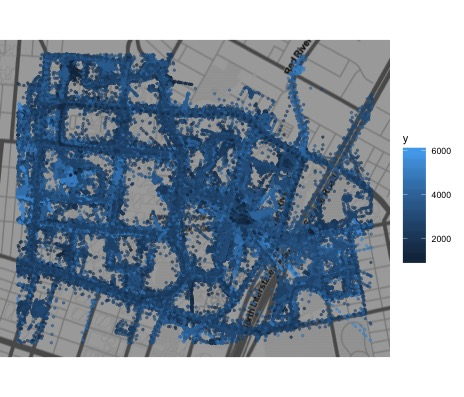
\includegraphics[width=0.7\columnwidth]{Images/original_data_plot.jpg}
\caption{Observed data.}
\label{fig:1}
\end{figure}

Second, Katzfuss and Cressie suggest de-trending to adjust for any large-scale spatial variation and any key covariates.  We plotted the raw data versus longitude, latitude, and temperature in Figure \ref{fig:2}.  The data do not show any trend by latitude or longitude, ruling out deterministic trends.  There is a trend by temperature, which is not surprising as lower temperatures may affect the accuracy of the radiation measurements. \\

We chose not to de-trend the data by temperature, as this introduced strange patterns in the data when plotted by latitude and longitude. \\

\begin{figure}[H]
\centering
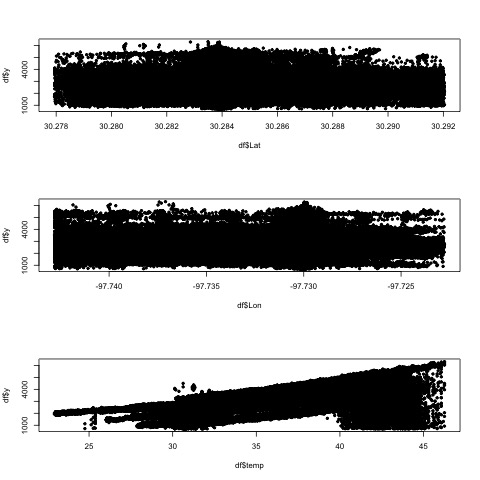
\includegraphics[width=0.45\columnwidth]{Images/detrending_plots.jpg}
\caption{Data by Latitude, Longitude and Temperature.}
\label{fig:2}
\end{figure}

\underline{Transformation to Normality}\\
Third, Katzfuss and Cressie recommend the data to be checked for approximate normality and transformed if necessary.  The radiation data is in the form of counts (intensity measurements) and is likely to be Poisson distributed, so we use an Anscombe transformation to induce normality.  A histogram of the normalized observations (see Figure \ref{fig:3}) confirms this transformation was successful.  Note that Anscombe back-transformations can lead to a biased result, and so we use the following transform and back-transform. \\

\myindent $x \rightarrow 2\sqrt{x + \frac{3}{8}}$\\
\myindent $y \rightarrow \left(\frac{y}{2}\right)^2 - \frac{1}{8}$ 
\myindent (instead of the direct algebraic inverse, where $\frac{3}{8}$ is subtracted.)

\begin{figure}[H]
\centering
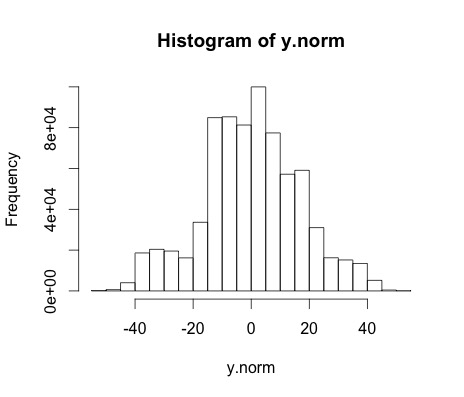
\includegraphics[width=0.5\columnwidth]{Images/histogram_ynorm}
\caption{Anscombe-Transformed Responses.}
\label{fig:3}
\end{figure}

\newpage
\subsection{Basis Function Generation}

The choice of the basis functions is a very important step in the model specification for FRK. In fact, the matrix $S$ allows us to represent the covariance structure as a linear combination of some basis function $S_1(\bm{u}), \dots, S_r(\bm{u})$, which results in a loss of information with respect to the full covariance representation. \\

The choice of the basis functions has to combine two goals. First of all, we should choose a number of basis functions $r \ll n$ in order to see an actual gain in terms of computational efficiency. Moreover, the basis functions have to be multiresolutional, that is, they should be allowed to capture multiple scales of variation in the covariance structure. In practice, there are a few smooth basis functions with large support (the limit case is the constant basis function, that is already implied in the centering step), and many spiky basis functions with small support. \\

The choice of the basis functions involves three separate problems: the choice of the \textit{type}, the \textit{number} $r$ and the \textit{locations}. The basis functions do not have to be necessarily orthogonal. In this work, we use bisquare functions, i.e. functions of the form
\begin{equation*}
f(r) = \begin{cases}
\left[ 1 - \left( \frac{r}{c} \right)^2 \right]^2 & r \leq c
\\
0 & r > c
\end{cases}
\end{equation*}
where $c$ represents the resolution of the function and $r$ is the euclidean distance of the coordinate from the center of the function. The number of basis functions $r$ is chosen heuristically, in such a way that it can represent well the domain but that it does not compromise the performance of the algorithm. As far as the locations are concerned, they should cover as much as possible the spatial domain of interest (the prediction grid), and they should not overlap for different basis functions.\\

In this work we use a total of $r = 50$ basis functions with three different resolutions. In particular, $r_1 = 9$ functions have a low resolution $c_1 = 10^{-2}$, $r_2 = 16$ functions have an intermediate resolution $c_2 = 7 \cdot 10^{-3}$ and $r_3 = 25$ functions have a high resolution $c_3 = 5 \cdot 10^{-3}$. In order to choose the basis resolution, we followed Cressie's rule, which consists in setting it equal to $1.5$ times the shortest distance between the centers of any of the functions with that resolution. In Figure \ref{fig:res1} - \ref{fig:res3} some examples of basis functions are illustrated.

\begin{figure}[H]
\centering
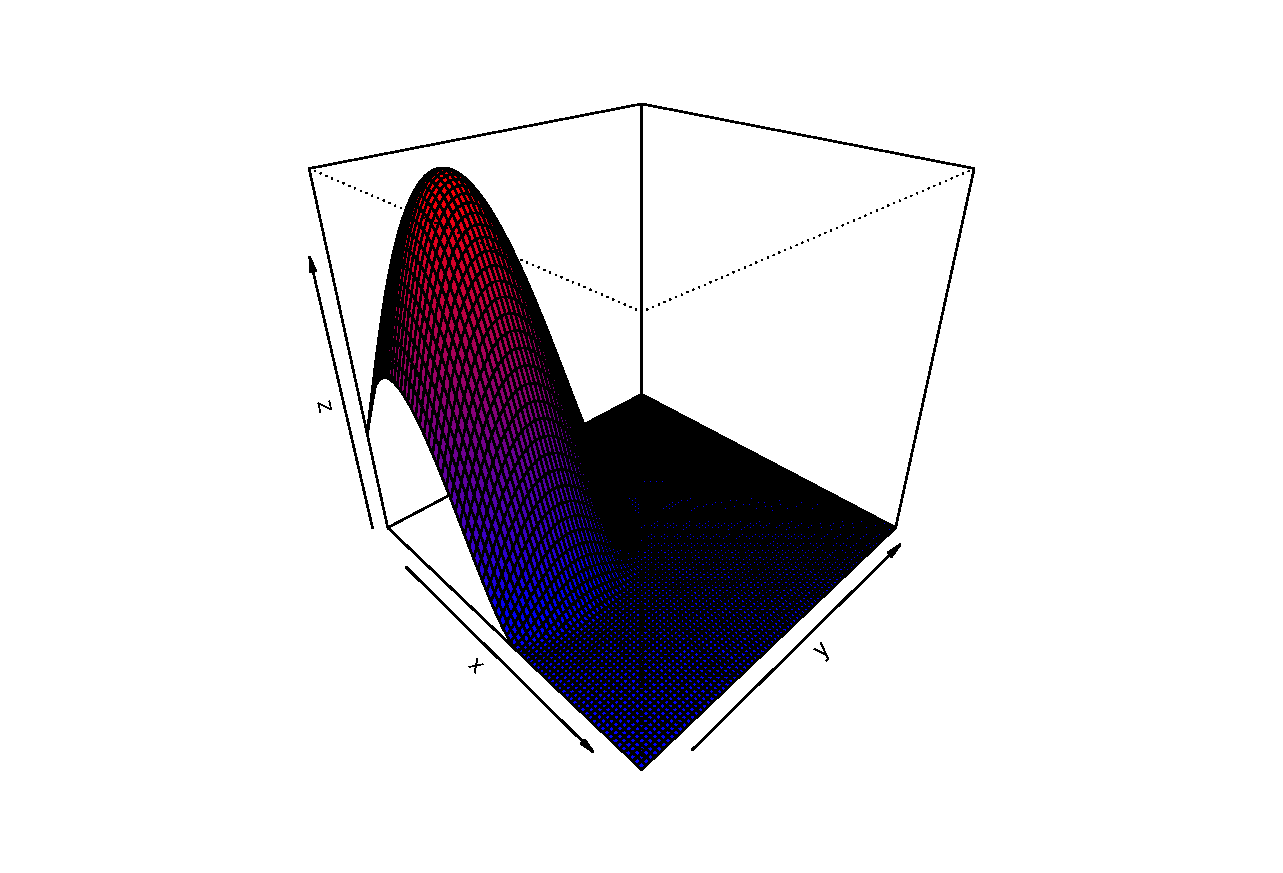
\includegraphics[width=0.55\columnwidth]{./Images/res1}
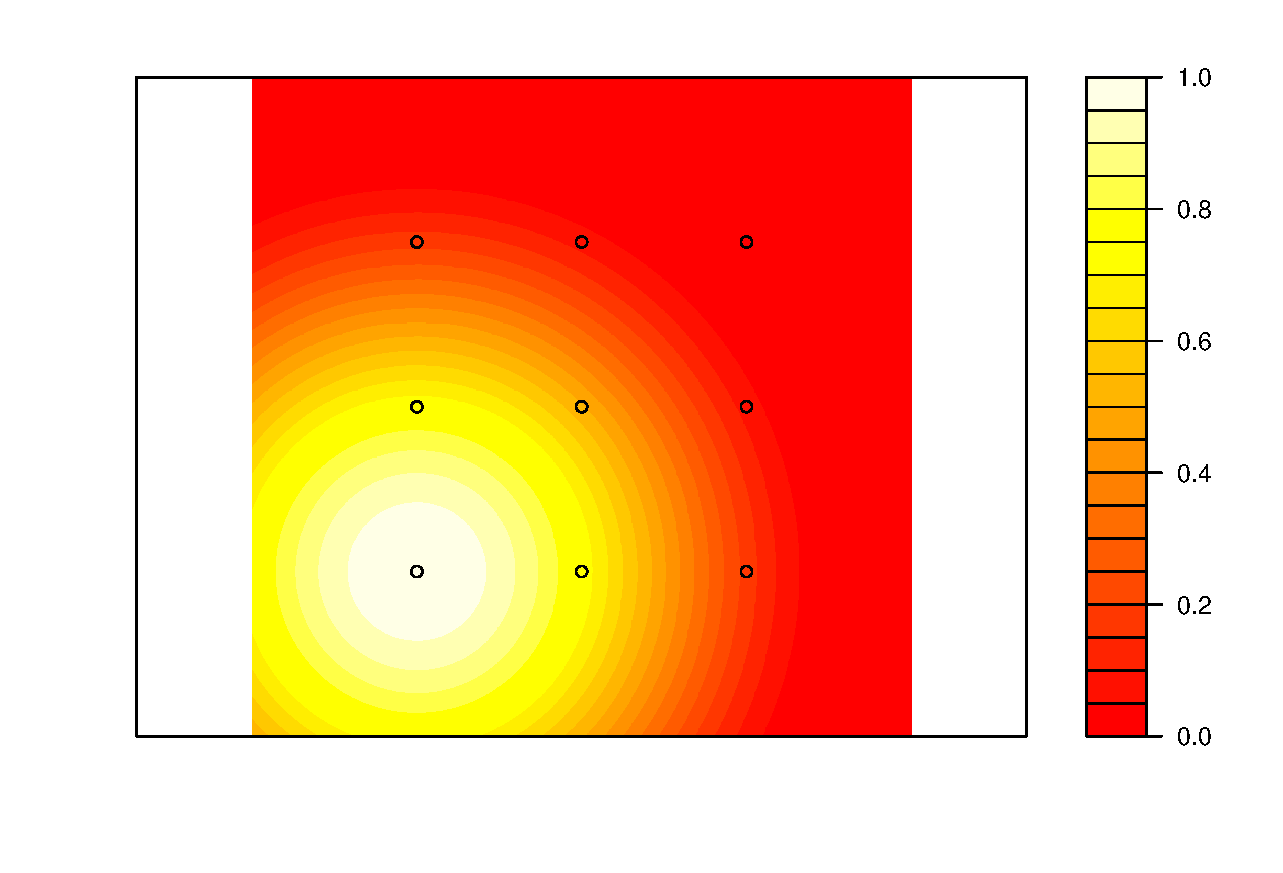
\includegraphics[width=0.44\columnwidth]{./Images/res11}
\caption{Example of low resolution basis function.}
\label{fig:res1}
\end{figure}

\begin{figure}[H]
\centering
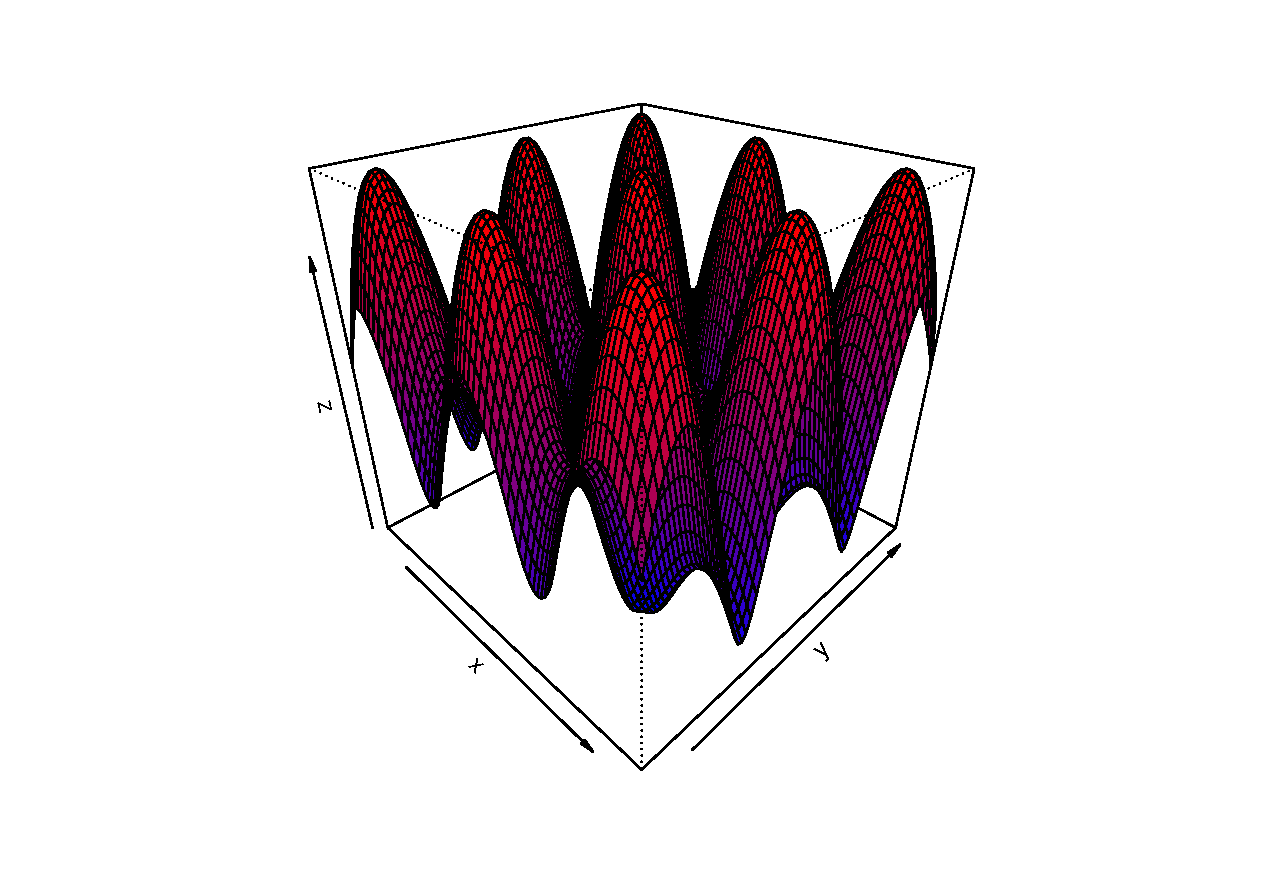
\includegraphics[width=0.55\columnwidth]{./Images/res2}
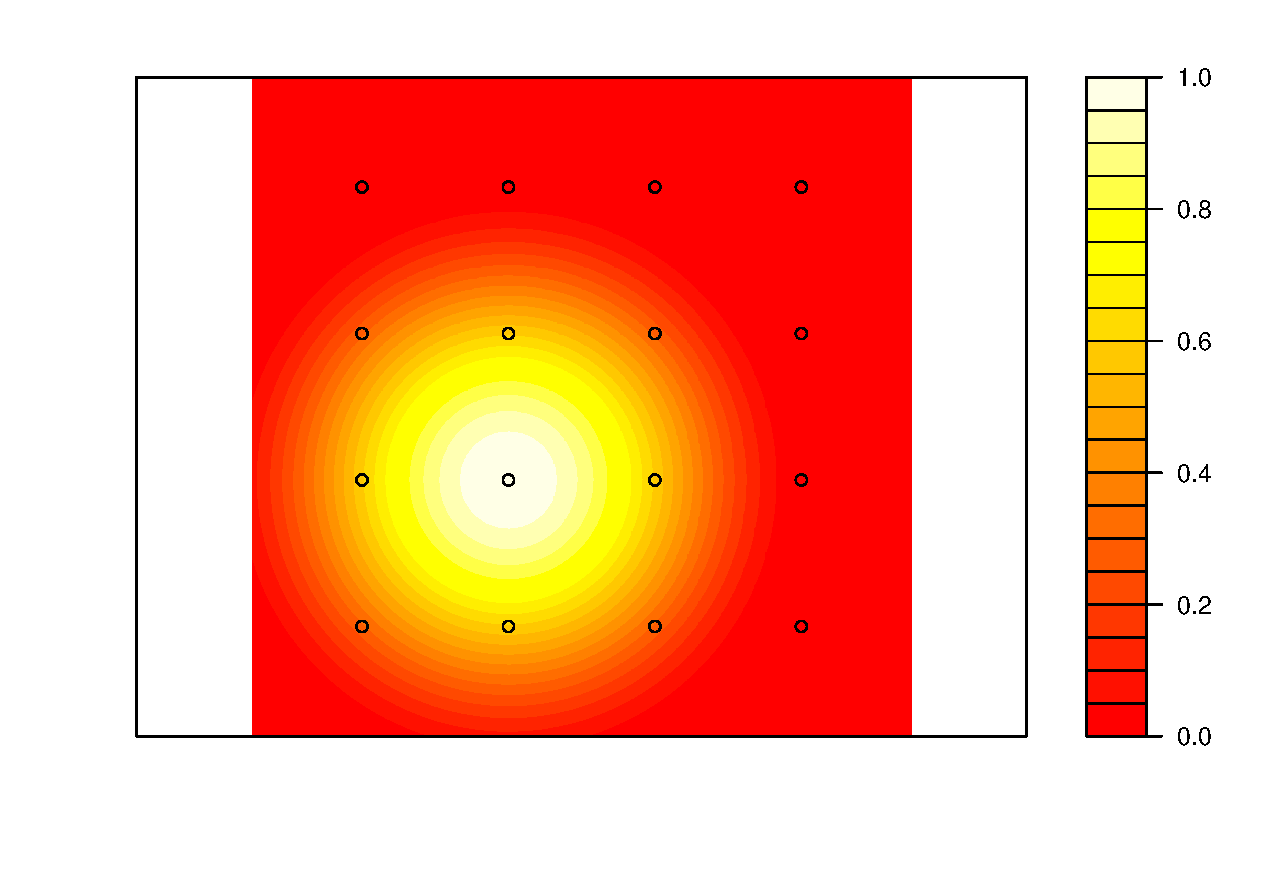
\includegraphics[width=0.44\columnwidth]{./Images/res21}
\caption{Example of intermediate resolution basis function.}
\label{fig:res2}
\end{figure}

\begin{figure}[H]
\centering
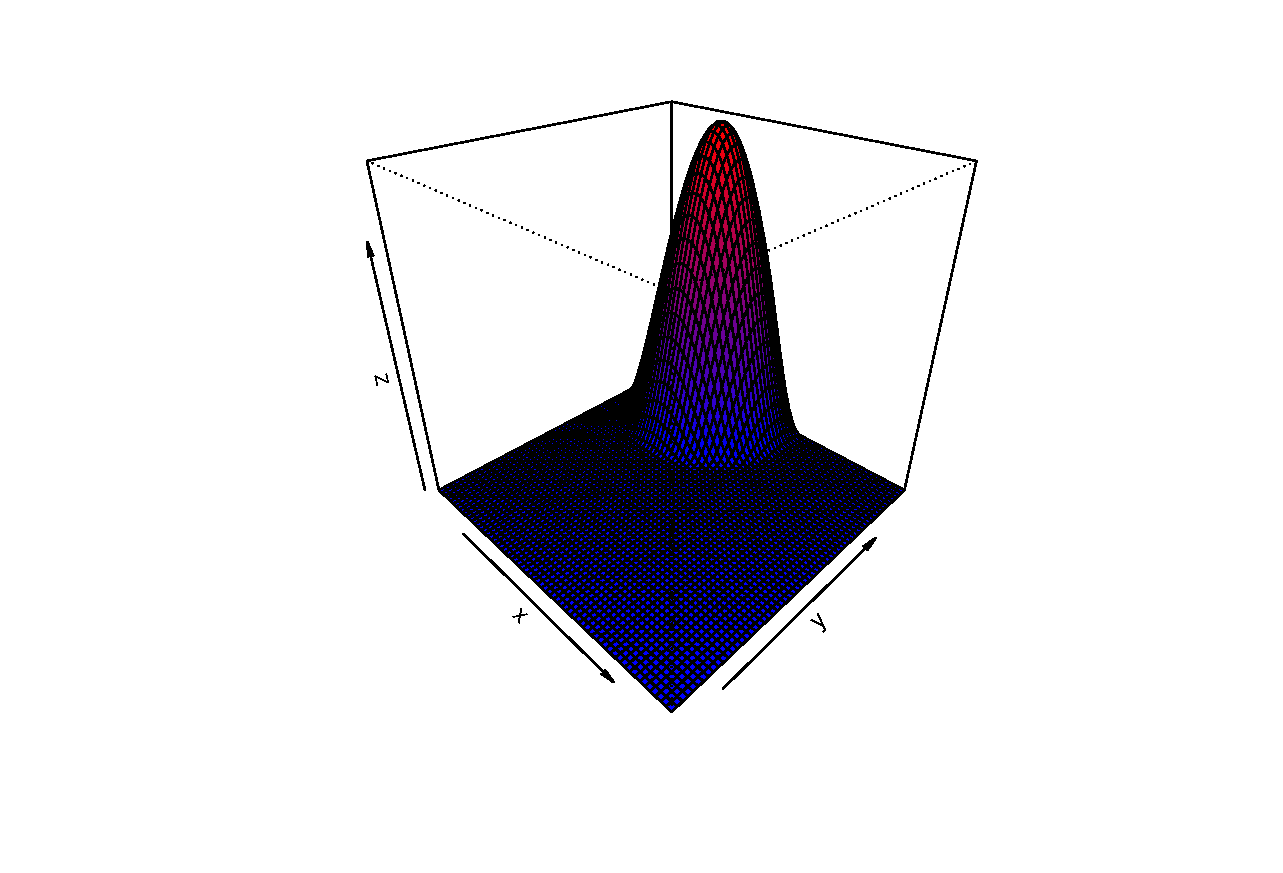
\includegraphics[width=0.55\columnwidth]{./Images/res3}
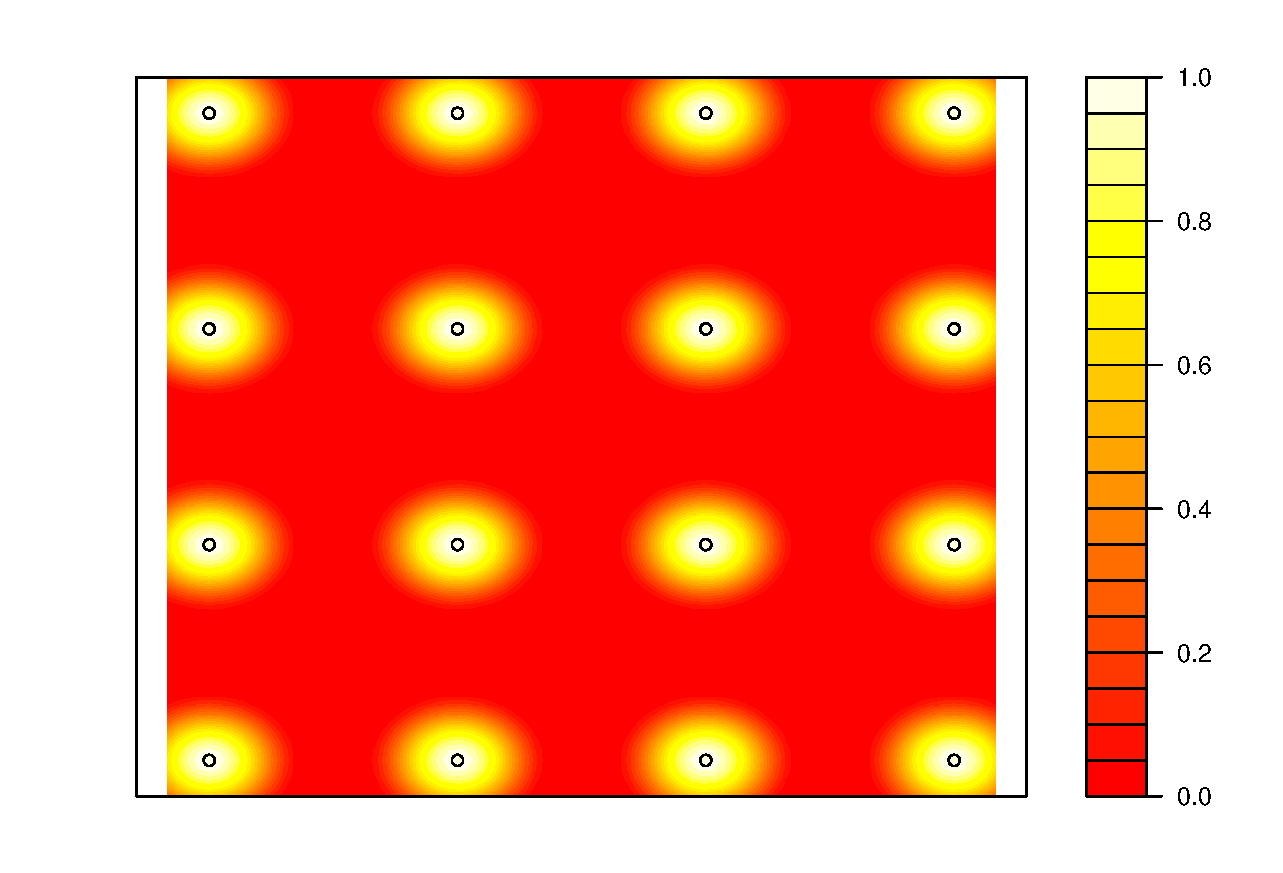
\includegraphics[width=0.44\columnwidth]{./Images/res31}
\caption{Example of high resolution basis function.}
\label{fig:res3}
\end{figure}

\subsection{Estimation of $\sigma^2_{\epsilon}$ via Semivariogram}

The FRK model specifies that $n$ measurements are modeled as $Z(s_i) = Y(s_i) + \epsilon(s_i)$, where $s_i$ are locations in the region of interest, and $\epsilon(s_i)$ is additive measurement error.\\

As detailed above, the measurement error is assumed to be independent of $Y(s_i)$ and normally distributed as $\epsilon(s_i) \sim N(0,\sigma^2_\epsilon v_\epsilon (s_i))$.  The $v_\epsilon (s_i)$ component is a function that is assumed to be known, which describes the random spatial variation.  As with the CO2 data, we assume $v_\epsilon (s_i)$ is a constant function equal to 1 at every location, as we assume that random spatial variation is constant over the campus. \\

This leaves us with $\sigma^2_\epsilon$ to estimate. Katzfuss and Cressie note that $\sigma^2_\epsilon$ may be specified in advance, if there is previous knowledge about measurement error for the instrument being used.  We do not assume prior knowledge of $\sigma^2_\epsilon$. \\

The semivariogram estimation method presented in Katzfuss and Cressie is known as the `Robust Cressie Variogram'.  \\

\myindent $\bullet$ $2\gamma(h) = \left( \frac{1}{|N(h)|} \sum_{N(h)} \biggr\rvert
\frac{\tilde{Z}(s_i)}{\sqrt{v_\epsilon (s_i)}} - 
\frac{\tilde{Z}(s_j)}{\sqrt{v_\epsilon (s_j)}} - 
\biggr\rvert^{1/2} \right)^4 / \left(0.457 + 0.494 / |N(h)|\right)$ \\

\myindent\myindent where: \\
\myindent \myindent  $\tilde{Z}(s_i)$ are the normalized, de-trended data. \\
\myindent \myindent $N(h) = {(i,j): ||s_i - s_j|| \in [h - \delta, h + \delta ] }$, \\
\myindent \myindent \myindent the set of all indices for location pairs roughly $h$ distance apart.\\

\myindent $\bullet$ Then straight line $\hat{\gamma}(h) = \hat{\gamma}(0) + bh$ is fit, and $\sigma^2_\epsilon = \hat{\gamma}(0)$.\\

For further detail on this methodology, see Cressie and Hawkins (1980), Cressie (1985), and Kang et al. (2010). We use this method to estimate a semi-variogram for the data, and then fit a straight line to the semivariogram and let $\hat{\sigma}^2_\epsilon$ be equal to the intercept.  Our resulting estimate is $\hat{\sigma}^2_\epsilon$ = 106.3635. \\

We did remove the police station measurements in the calculation of this semivariogram.  The police car carrying the measurement device parked in the police station lot overnight, so there were a disproportionate number of measurements at this location, including specifically night-time measurements where cooler temperatures mean the measurement device is more prone to error. \\

Our estimate was considerably higher than the estimate obtained for the Katzfuss and Cressie simulated CO2 data.  However, their data was simulated with $\sigma^2_\epsilon = 0.25$. Our normalized data, instead, has a range of $-51$ to $54$, with a total variance of around $287$, so our result is reasonable. To check reasonableness, we split the region of interest into four quadrants and calculated semivariograms for each quandrant to ensure that they yielded comparable $\hat{\sigma}^2_\epsilon$ estimates. Estimates were similar in all regions, and did not differ significantly from the overall estimate.   The data is known to have some outliers which affect the variance.\\


\subsection{Estimation of $\sigma^2_{\xi}$ and $K$ via EM Algorithm}

The next step of the Fixed Rank Kriging process is to estimate the parameters $\sigma^2_{\xi}$ and $K$.  \\

As described above, $K$ is the $r \times r$ covariance matrix, where $r$ is the number of basis functions selected.  $K$ represents the covariance in the spatial-random-effects (SRE) model. $\sigma^2_{\xi}$ is the fine-scale variance in the SRE model, accounting for error introduced to the model through the dimension reduction. \\

Katzfuss and Cressie suggest two methods for estimating these parameters: the method of Moments and the EM Algorithm.  We have implemented the EM algorithm to estimate these values.\\

\myindent $\bullet$ Begin with default choices suggested in Katzfuss and Cressie: \\

\myindent \myindent $K^{[0]} = (0.9)\nu ^2 I_r$ \\
\myindent \myindent $\sigma_\xi^{2[0]} = (0.1)\nu ^2 I_r$ \\
\myindent \myindent \myindent where $\nu^2 = \tilde{\bm{Z}}^T\tilde{\bm{Z}}/n$.\\

\myindent $\bullet$ Iteratively update the two parameters until convergence is met:\\

\myindent \myindent $K^{[t+1]} = K^{[t]} - K^{[t]} S^T \Sigma^{[t]-1}SK^{[t]}
  + \left(K^{[t]}S^T \Sigma^{[t]-1} \tilde{\bm{Z}} \right)\left(K^{[t]}S^T \Sigma^{[t]-1} \tilde{\bm{Z}} \right)^T$ \\
\myindent \myindent $\sigma_\xi^{2[t+1]} = \sigma_\xi^{2[t]} + \left(\sigma_\xi^{2[t]} \right)^2 \text{tr} \left(\Sigma^{[t]-1}[\tilde{\bm{Z}}\tilde{\bm{Z}}^T\Sigma^{[t]-1} - \mathcal{I}_n]V_\xi \right)$\\

\underline{Computational notes:} \\
\myindent $\bullet$ $\Sigma^{[t]-1}$ is shorthand for $(\Sigma^{[t]})^{-1}$ \\
\myindent $\bullet$ As discussed previously, we used the Sherman-Morrison-Woodbury formula to  \\ \myindent \myindent efficiently compute $\Sigma^{[t]-1}$.\\
\myindent $\bullet$ So we let $D^{[t]} = \sigma^{2[t]}V_\xi + \sigma^2_\epsilon V_\epsilon$. \\
\myindent $\bullet$ Then $\Sigma^{[t]-1} = D^{[t]-1} -  D^{[t]-1}S[K^{[t]-1} + SD^{[t]-1}S]^{-1}S^TD^{[t]-1}$\\

We can use these results to re-write the $\sigma_\xi^{2[t+1]}$ update in a more efficient way: \\

\myindent \myindent $\sigma_\xi^{2[t+1]} = \sigma_\xi^{2[t]} 
+ \left( \sigma_\xi^{2[t]} \right)^2 \text{tr} \left([S^TD^{[t]-1}V_\xi D^{[t]-1}S][K^{[t]-1} + S^TD^{[t]-1}S]^{-1} \right)/n \\ \myindent \myindent \myindent
- \left( \sigma_\xi^{2[t]} \right)^2 \text{tr}(D^{[t]-1}V_\xi)/n
+ \left(\sigma_\xi^{2[t]}V_\xi \Sigma^{[t]-1} \tilde{\bm{Z}}\right)^T
V_\xi^{-1}
\left(\sigma_\xi^{2[t]}V_\xi \Sigma^{[t]-1} \tilde{\bm{Z}}\right)/n$\\


\underline{Results:}\\
We obtain an estimated $\hat{\sigma}^2_{\xi} = 174.4245$.  The R code saves $\hat{\sigma}^2_{\xi}$ and $\hat{K}$ as part of the EM function output.\\

\subsection{Fixed Rank Kriging: Smoothing and Prediction}

We implemented the Fixed Rank Kriging process using the equations described previously.

\begin{equation}
\hat{Y}(\bm{s}^*) = \bm{t}(\bm{s}^*)^T \hat{\bm{\alpha}} + \bm{S}(\bm{s}^*)^T K S^T \Sigma^{-1} (\bm{Z} - T \hat{\bm{\alpha}}), \quad \bm{s}^* \in \mathbb{R}^2
\end{equation}
and the standard error is
\begin{equation}
\begin{split}
\sigma_k(\bm{s}^*) = \big[ &\bm{S}(\bm{s}^*)^T K \bm{S}(\bm{s}^*) - \bm{S}(\bm{s}^*)^T K S^T \Sigma^{-1} S K \bm{S}(\bm{s}^*) + 
\\
&+ (\bm{t}(\bm{s}^*) - T^T \Sigma^{-1} S K \bm{S}(\bm{s}^*))^T (T^T \Sigma^{-1} T)^{-1} (\bm{t}(\bm{s}^*) - T^T \Sigma^{-1} S K \bm{S}(\bm{s}^*)) \big]^{1/2}
\end{split}
\end{equation}

where $\Sigma = S K S^T + D = S K S^T + (\sigma_\epsilon^2 + \sigma_\xi^2) \mathcal{I}_n$.\\

The Kriging function returns a grid of locations and estimated responses, along with a vector of kriging variances.  Results are included in subsequent sections. \\

%%%%%%%%%%%%%%%%%%%%%%%%%%%%%%%%%%%%%%%%%%%%%%%%%%%%%%%%%%%%%%%%%%%%
%%                     RESULTS                                    %%
%%%%%%%%%%%%%%%%%%%%%%%%%%%%%%%%%%%%%%%%%%%%%%%%%%%%%%%%%%%%%%%%%%%%
\newpage
\section{3. Results}

Using a the uniform set of basis functions presented in the previous section, predicted kriging values are shown in Figure \ref{fig:4}, followed by a plot of the kriging variance in Figure \ref{fig:5}. 

\begin{figure}[H]
\centering
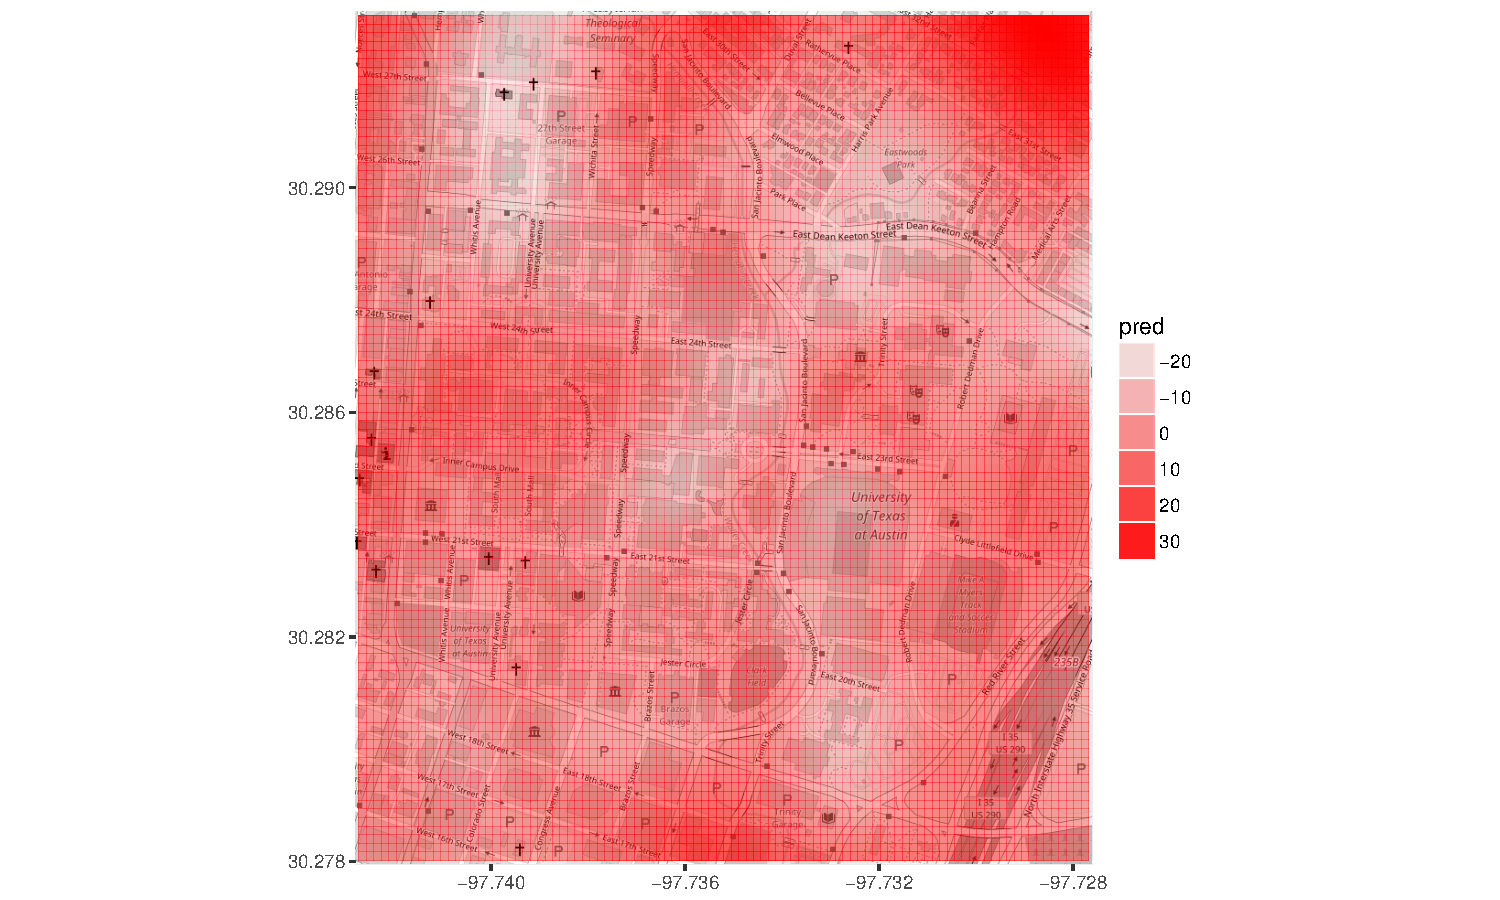
\includegraphics[width=0.8\columnwidth]{Images/pred.pdf}
\caption{Predicted values, uniform basis.}
\label{fig:4}
\end{figure}

\begin{figure}[H]
\centering
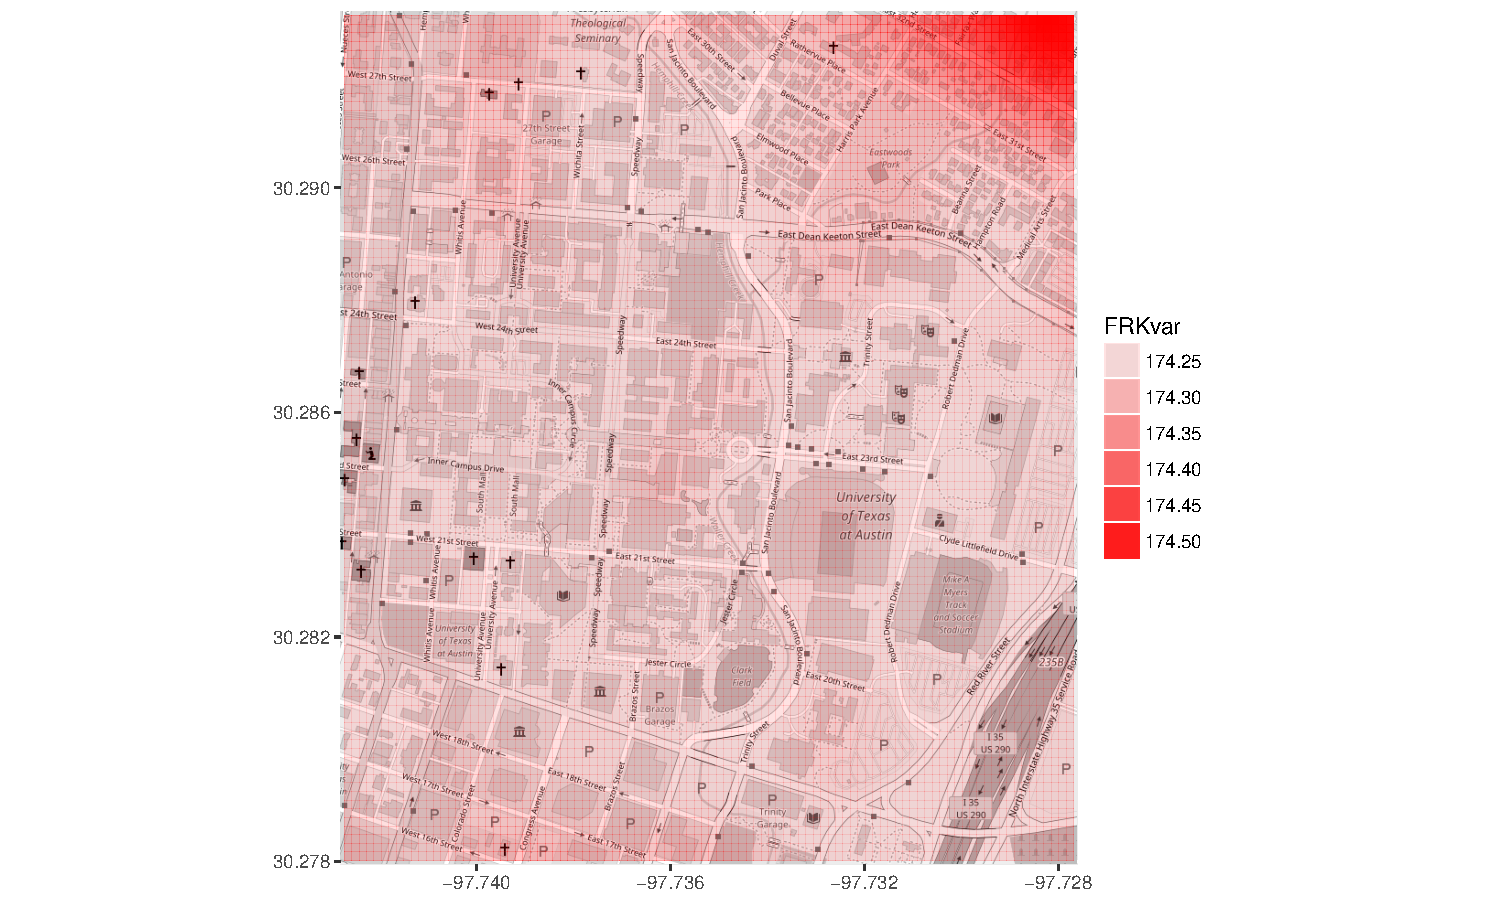
\includegraphics[width=0.8\columnwidth]{Images/var.pdf}
\caption{FRK variance, uniform basis.}
\label{fig:5}
\end{figure}

\begin{figure}[H]
\centering
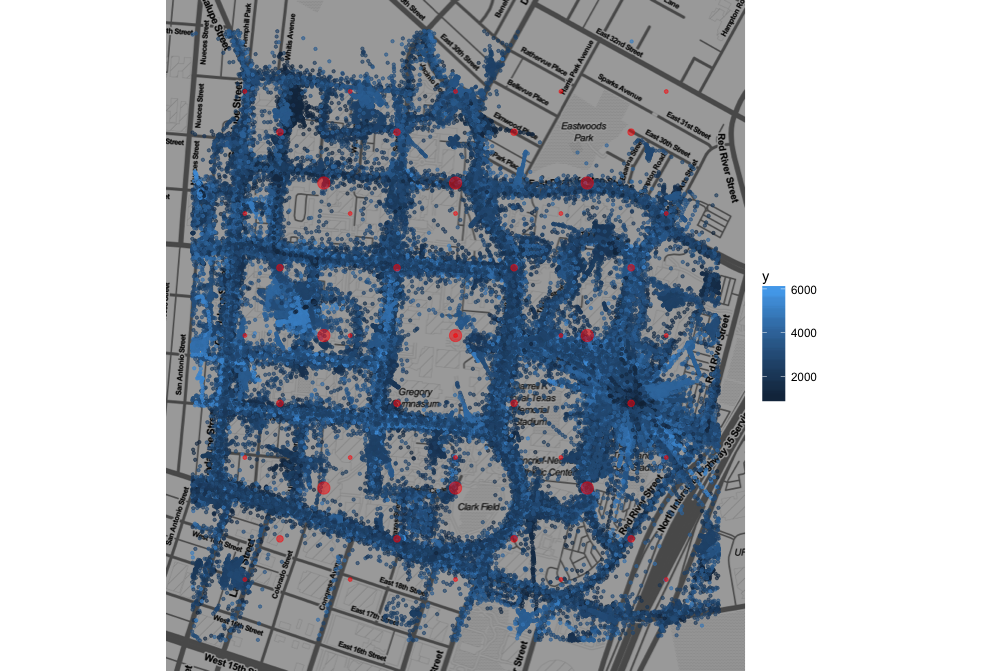
\includegraphics[width=0.8\columnwidth]{Images/data_grid}
\caption{Observed data are plotted in different shades of blue, according to their intensity. The centers of the basis function are displayed in red. The size of the dots denotes the resolution of the function (the bigger the dot, the lower the resolution).}
\label{fig:6}
\end{figure}

We noticed an area in the top right of very high variance.  This issue is caused by very sparse observed data coverage in the top right area of the grid; there is one blue point by itself which is near East 32nd Street.  There are no other close points informing the kriging estimate in this area of the grid, and compounding the issue, there are two spiky basis centers quite close to this point. \\

To address this issue, we adjusted the basis centers by removing the two spiky centers in this corner.  We justified this by noting that kriging is not intended to extrapolate into new regions without surrounding estimates to inform the prediction.  Of course a lone point is going to have a high kriging variance, when none of its neighbors are near. The result of this adjustment is presented in Figure \ref{fig:7} - \ref{fig:9}.

\begin{figure}[H]
\centering
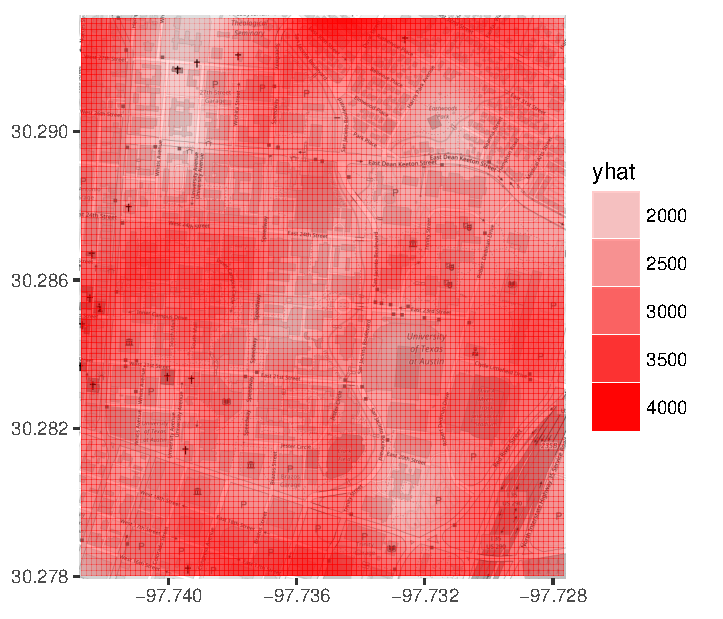
\includegraphics[width=0.8\columnwidth]{Images/pred_newgrid_origscale.pdf}
\caption{Predicted values, adjusted basis.}
\label{fig:7}
\end{figure}

\begin{figure}[H]
\centering
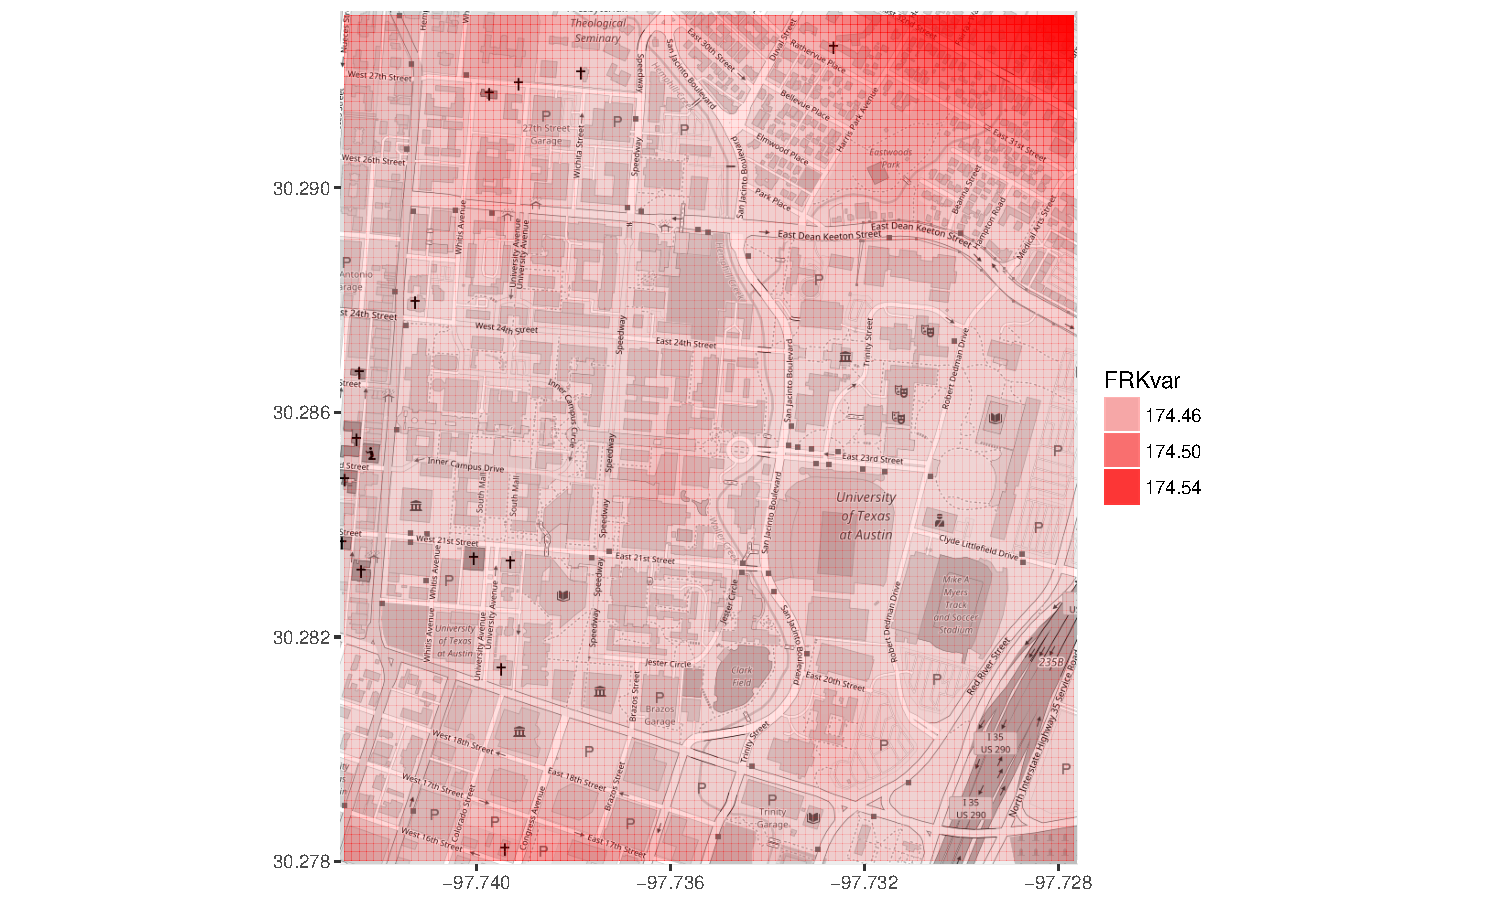
\includegraphics[width=0.8\columnwidth]{Images/var_newgrid.pdf}
\caption{FRK variance, adjusted basis.}
\label{fig:8}
\end{figure}

\begin{figure}[H]
\centering
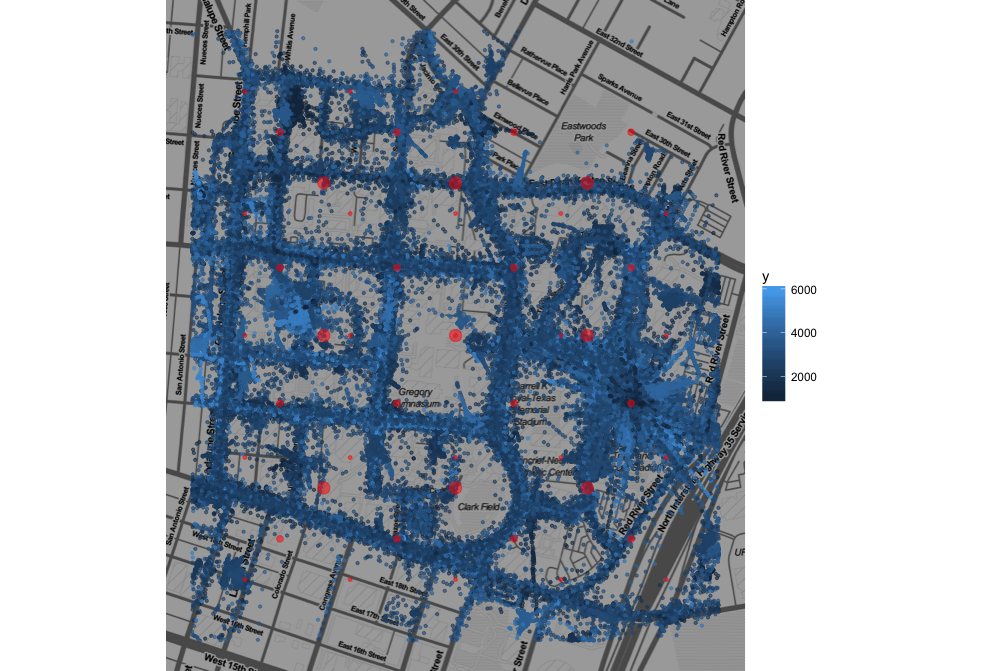
\includegraphics[width=0.8\columnwidth]{Images/data_grid_new.png}
\caption{Observed data are plotted in different shades of blue, according to their intensity. The centers of the basis function are displayed in red. The size of the dots denotes the resolution of the function (the bigger the dot, the lower the resolution).}
\label{fig:9}
\end{figure}

The result of this adjustment yields desirable results for the predicted data. The kriging variance is nearly uniform across the predicted grid of locations, with the area of high variance in the top right region reduced in size.\\

Finally, in Figure \ref{fig:10}, we include a histogram of the observed versus predicted residual for the kriging function applied to the observed locations.  These values should be normally distributed to indicate goodness of model fit.

\begin{figure}[H]
\centering
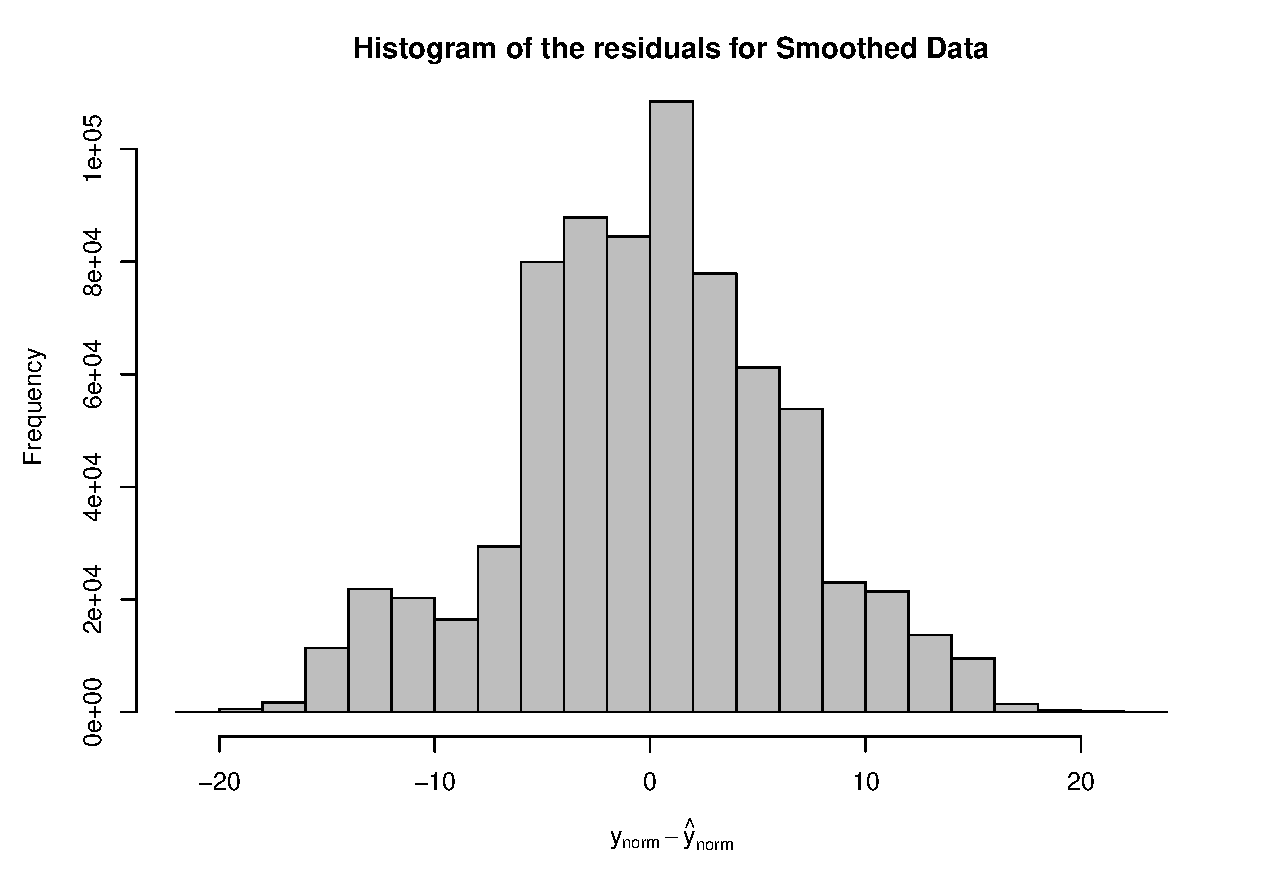
\includegraphics[width=0.5\columnwidth]{Images/Residuals_for_smoothing}
\caption{Histogram of the residuals.}
\label{fig:10}
\end{figure}


%%%%%%%%%%%%%%%%%%%%%%%%%%%%%%%%%%%%%%%%%%%%%%%%%%%%%%%%%%%%%%%%%%%%
%%                     DISCUSSION                                 %%
%%%%%%%%%%%%%%%%%%%%%%%%%%%%%%%%%%%%%%%%%%%%%%%%%%%%%%%%%%%%%%%%%%%%
\newpage
\section{4. Discussion}

Our Fixed Rank Kriging results looked to be reasonable based on comparison with the underlying observed data, our knowledge of potential higher-radiation areas on campus, and based on the normality of the histogram of the residuals.  Our code was computationally efficient, executing the entire process including semivariogram estimation, basis function generation, EM algorithm calculations, and Fixed Rank Kriging computations in 18 minutes.\\

To increase efficiency over a large data set, our implementation uses pre-caching and sparse matrix functionality to the extent possible.  $D^{-1}$ is stored as a sparse matrix since it is diagonal.  Computations involving matrix multiplications that always appear together in updates are pre-cached, such as $K^{[t]}S^T\Sigma^{[t]-1}$.\\

One limitation in our code is the calculation of the Fixed Rank Kriging variance in the case where the code is run for smoothing the observed values, instead of predicting over a grid of new values.  We omitted the computation of the Fixed Rank Kriging variance in the case where the function is smoothing, ie 100\% of the locations to be predicted correspond with already-observed locations.  The variance computation becomes very computationally intensive in this case, and a future area for expansion is to implement the FRK variance calculation in C++.\\

%%%%%%%%%%%%%%%%%%%%%%%%%%%%%%%%%%%%%%%%%%%%%%%%%%%%%%%%%%%%%%%%%%%%
%%                     R APPENDIX & DOCUMENTATION                 %%
%%%%%%%%%%%%%%%%%%%%%%%%%%%%%%%%%%%%%%%%%%%%%%%%%%%%%%%%%%%%%%%%%%%%
\newpage
\section{5. R Code Appendix}

\subsection{Documentation Source}
All project documentation and source code is available in the following github repository.\\

\myindent \url{https://github.com/jstarling1/spatialsmoothing}\\

The R code launcher is available in the \textit{R Code\_Launcher} directory.\\

\end{document}